% This is file JFM2esam.tex
% first release v1.0, 20th October 1996
% release v1.01, 29th October 1996
% release v1.1, 25th June 1997
% release v2.0, 27th July 2004
% (based on JFMsampl.tex v1.3 for LaTeX2.09)
% Copyright (C) 1996, 1997 Cambridge University Press

\NeedsTeXFormat{LaTeX2e}

\documentclass{jfm}%

\usepackage{graphicx}%
\usepackage{natbib}%
\usepackage{amsbsy}%
%\usepackage{upmath}%
\usepackage{amssymb}%
\usepackage{amsmath}%
\usepackage{subcaption}
\usepackage{import}
\usepackage[usenames,dvipsnames]{xcolor}
\usepackage[nolist,nohyperlinks]{acronym}
\usepackage{snapshot}
\usepackage{comment}
\usepackage{booktabs}
\usepackage{multicol}
\usepackage{soul}
\usepackage{array}
\usepackage{tikz}
\newcolumntype{L}[1]{>{\raggedright\let\newline\\\arraybackslash\hspace{0pt}}m{#1}}
\newcolumntype{C}[1]{>{\centering\let\newline\\\arraybackslash\hspace{0pt}}m{#1}}
\newcolumntype{R}[1]{>{\raggedleft\let\newline\\\arraybackslash\hspace{0pt}}m{#1}}

%%% example macros (some are not used in this sample file) %%%

% for units of measure
\newcommand\dynpercm{\nobreak\mbox{$\;$dyn\,cm$^{-1}$}}
\newcommand\cmpermin{\nobreak\mbox{$\;$cm\,min$^{-1}$}}

% various bold symbols
\newcommand{\bs}[1]{\boldsymbol{#1}}
\providecommand\bnabla{\boldsymbol{\nabla}}
\providecommand\bcdot{\boldsymbol{\cdot}}

% for multiletter symbols
\newcommand\real{\mbox{re}} % cf plain tex's \re and reynolds number
\newcommand\imag{\mbox{im}} % cf plain tex's \im
\newcommand\rey{\mbox{\textit{re}}}  % reynolds number
\newcommand\pran{\mbox{\textit{pr}}} % prandtl number, cf tex's \pr product
\newcommand\pen{\mbox{\textit{pe}}}  % peclet number
\newcommand\ai{\mbox{ai}}            % airy function
\newcommand\bi{\mbox{bi}}            % airy function

% for sans serif characters:
% the following macros are setup in jfm.cls for sans-serif fonts in text
% and math.  if you use these macros in your article, the required fonts
% will be substitued when you article is typeset by the typesetter.% 
% \textsfi, \mathsfi   : sans-serif slanted
% \textsfb, \mathsfb   : sans-serif bold
% \textsfbi, \mathsfbi : sans-serif bold slanted (doesnt exist in cm fonts)
% 
% for san-serif roman use \textsf and \mathsf as normal.
% 
\newcommand\ssc{\mathsf{c}}    % for sans serif c
\newcommand\sfsp{\mathsfi{p}}  % for sans serif sloping p
\newcommand\slsq{\mathsfbi{q}} % for sans serif bold-sloping q

% hat position
\newcommand\hatp{\skew3\hat{p}}      % p with hat
\newcommand\hatr{\skew3\hat{r}}      % r with hat
\newcommand\hatrr{\skew3\hat{\hatr}} % r with 2 hats
\newcommand\doubletildesigma{\skew2\tilde{\skew2\tilde{\sigma}}}
% italic sigma with double tilde

% array strut to make delimiters come out right size both ends
\newsavebox{\astrutbox}
\sbox{\astrutbox}{\rule[-5pt]{0pt}{20pt}}
\newcommand{\astrut}{\usebox{\astrutbox}}

\newcommand\gapq{\ensuremath{g_a(p,q)}}
\newcommand\gspq{\ensuremath{g_s(p,q)}}
\newcommand\p{\ensuremath{\partial}}
\newcommand\tti{\ensuremath{\rightarrow\infty}}
\newcommand\kgd{\ensuremath{k\gamma d}}
\newcommand\shalf{\ensuremath{{\scriptstyle\frac{1}{2}}}}
\newcommand\sh{\ensuremath{^{\shalf}}}
\newcommand\smh{\ensuremath{^{-\shalf}}}
\newcommand\squart{\ensuremath{{\textstyle\frac{1}{4}}}}
\newcommand\thalf{\ensuremath{{\textstyle\frac{1}{2}}}}
\newcommand\gat{\ensuremath{\widetilde{g_a}}}
\newcommand\ttz{\ensuremath{\rightarrow 0}}
\newcommand\ndq{\ensuremath{\frac{\mbox{$\partial$}}{\mbox{$\partial$} n_q}}}
\newcommand\sumjm{\ensuremath{\sum_{j=1}^{m}}}
\newcommand\pvi{\ensuremath{\int_0^{\infty}%
    \mskip \ifcupmtlplainloaded -30mu\else -33mu\fi -\quad}}

\newcommand\etal{\mbox{\textit{et al.}}}
\newcommand\etc{etc.\ }
\newcommand\eg{e.g.\ }


\newtheorem{lemma}{lemma}
\newtheorem{corollary}{corollary}




% My math symbols
\newcommand{\orderof}[1]{\ensuremath{\textit{O}\left(#1\right)}}
\newcommand{\abs}[1]{\ensuremath{\left|#1\right|}}
\newcommand{\norm}[1]{\ensuremath{\left\Vert#1\right\Vert}}
\newcommand{\plus}{\raisebox{.2\height}{\scalebox{.8}{+}}}


% Fix subref format to include parentheses
\captionsetup{subrefformat=parens}

%%%%%%%%%%%%%%%%%%%%%%%%%%%%%%%%%%%%%%%%%%%%%%%%%%%%%%%%%% 


\title[]{Growth of liquid-gas interfacial perturbations driven by acoustic waves}

\author[B. Patterson and E. Johnsen]%
{Brandon Patterson$^1$ and %
  Eric Johnsen$^1$\thanks{Email address for correspondence: ejohnsen@umich.edu}\ns
}

% note: a full address must be provided: department, university/institution, town/city, zipcode/postcode, country.
\affiliation{$^1$Department of Mechanical Engineering, University of Michigan,
  Ann Arbor, MI 48109, USA}

\pubyear{2010}
\volume{650}
\pagerange{119--126}
% do not enter received and revised dates. these will be entered by the editorial office.
\date{?; revised ?; accepted ?. - to be entered by editorial office}
% \setcounter{page}{1}
\begin{document}

\maketitle

% Define acronyms used in this paper
\begin{acronym}
  \acro{DG}{Discontinuous Galerkin}
  \acro{US}{ultrasound}
  \acro{DUS}{Diagnostic ultrasound}
  \acro{HIFU}{High Intensity Focused Ultrasound}
  \acro{RM}{Richtmyer-Meshkov}
  \acro{RT}{Rayleigh-Taylor}
\end{acronym}

\begin{abstract}
  Diagnostic ultrasound has been shown to cause lung hemorrhage in a
  variety of mammals, though the underlying damage mechanisms are
  still unclear. Motivated by this problem, we use numerical
  simulations to investigate the interaction of an ultrasound wave
  with the alveolar tissue-air interface. A planar, positive, trapezoidal waveform
  propagates in tissue (modelled as water) and
  impinges upon an alveolus of the lung (modelled as air); to
  represent the alveolar surface roughness, the interface consists of a
  small-amplitude, single-mode perturbation. Because of the sharp
  density gradient at the interface, we hypothesize that ultrasound
  waves, despite their relatively low amplitude, deposit sufficient
  baroclinic vorticity to drive perturbation growth. Our simulations
  show that the perturbation amplitude grows to sizes many times
  larger than the original value, \emph{well after the wave has
    passed}. We demonstrate that conventional (linear) acoustics
  cannot account for such deformations; instead, the perturbation
  growth is driven by nonlinear effects---the baroclinic vorticity
  deposited along the interface, due to the misalignment of the
  pressure gradient (across the wave) and the density gradient (across
  the perturbed liquid-gas interface). Based on dimensional analysis
  and scaling, we observe that the perturbation amplitude and length of the
  interface scale with the circulation density and grow according to
  power laws in time. If the time-interval between the pressure increase
  and decrease is sufficient, both deposit vorticity of the same sign,
  thus enhancing the perturbation growth; conversely, if the interval
  is too short, the vorticity deposited by the pressure increase is
  canceled by the decrease. A further consequence is that one may be
  able to control the growth of such perturbed interfaces by
  modulating the incoming wave.
\end{abstract}

\begin{keywords}
\end{keywords}

\section{Introduction}%
\label{sec:introduction}%
% 
\ac{DUS} is one of the safest forms of medical imaging and has become
ubiquitous in clinical practice. \ac{DUS}-induced lung hemorrhage is
the only known bioeffect of non-contrast, pulsed \ac{US}, as bleeding
has been shown to occur in mammals including mice, rats, rabbits, pigs
and monkeys \citep{Child1990,OBrien2006a,Tarantal1994a,Miller2012}.
Furthermore, this problem has been shown to occur for a wide range of
frequencies from $1.5$ to $12$ MHz, for Mechanical indices well below
the accepted safe limit for diagnostic ultrasound, $\mbox{MI}=1.9$
\citep{OBrien2007}. Although this problem does not appear to be of
medical safety concern for humans under typical conditions, there is a
need to better understand the physical mechanisms of \ac{DUS}-induced
lung hemorrhage, which cannot currently be explained by
well-established \ac{US} bioeffects mechanisms. Typically, \ac{US}
bioeffects are generally classified as thermal or non-thermal, with
the bulk of non-thermal bioeffects being a result of acoustically
driven inertial cavitation. Except for one study reporting cavitation
activity \citep{Holland1996}, the bulk of the research suggests that
inertial cavitation is not the cause of \ac{DUS}-induced lung
hemorrhage: \cite{Raeman1996} and \cite{OBrien2004} found that
bleeding is not worsened by the use of ultrasound contrast agents, and
\cite{OBrien2000} observed that the severity of the hemorrhage
increases when the hydrostatic pressure is raised.  Beyond lung
hemorrhage, a number of studies have explored nonlinear mechanisms as
a potential cause for bioeffects. \cite{Filonenko2001} developed
numerical models to study the effects of acoustic nonlinearity on wave
propagation and heating in soft tissue. \cite{Khokhlova2006}
numerically solved a KZK-type equation simulating \ac{HIFU} fields in
a tissue phantom with the purpose of studying the impact of nonlinear
propagation, cavitation and boiling on lesion formation. Based on
potential flow simulations of an inviscid free surface subjected to a
Gaussian velocity potential, \cite{Tjan2007} suggested another damage
mechanism for \ac{DUS}-induced lung hemorrhage, namely that under the
right circumstances, droplets capable of puncturing the air-filled
sacs within the lung may be ejected by the focused
\ac{US}. \cite{Simon2012} experimentally demonstrated atomization of
water and soft tissue at air interfaces exposed to 2 MHz \ac{HIFU},
though at amplitudes higher than diagnostic. Despite these efforts,
the precise damage mechanism underlying \ac{DUS}-induced lung
hemorrhage is still unknown.

In parallel, the dynamics of accelerated interfaces separating fluids
of different densities have been the subject of intensive studies in
fluid mechanics. When exposed to accelerations whose sign is opposite
that of the density gradient, interfacial perturbations grow
exponentially as a manifestation of the Rayleigh-Taylor (RT)
instability \citep{Taylor1950}. Bubbles of light fluids ``rise'' into
the heavy fluid while spikes of heavy fluid ``fall'' into the light
fluid. Although the original analysis pertained to perturbation growth
at early times under constant acceleration, extensions to nonlinear
growth and time varying accelerations have been performed. In the
limit of instantaneous acceleration (e.g., as produced by a shock
wave), perturbations initially grow linearly in time, as predicted by
Richtmyer-Meshkov (RM) analysis \citep{Richtmyer1960, Meshkov1969},
regardless of the sign of the density gradient. To characterize the
growth at later times, \cite{Hecht1994} developed a potential flow
model for both RT and RM flows with Atwood Number
$A=\frac{\rho_{heavy}-\rho_{light}}{\rho_{heavy}+\rho_{light}}=1$,
which describes bubble growth in both linear and nonlinear regimes;
\cite{Srebro2003} extended this model to time-dependent Atwood numbers
and acceleration profiles. In both RT and RM flows, perturbation
growth can be explained by vorticity generated baroclinically, i.e.,
due to the misalignment of the density and pressure gradients:
\begin{align}
  \label{eq:baroclinic_equation}
  \frac{d\boldsymbol{\omega}}{dt} \biggr\rvert_{baroclinic} = \frac{\nabla \rho \times \nabla p}{\rho^2},%
\end{align}
where $\boldsymbol{\omega}$ is the vorticity, $\rho$ density and $p$
pressure. The majority of RT research has examined interfacial
perturbation growth under constant acceleration fields; RM research is
primarily concerned with shock-accelerated interfaces, where the
post-shock pressure is kept raised
\citep{Brouillette2002}. \citep{Jacobs1996} bouncing fluid tank to
experimentally study the RM instability between two liquids with an
initial interface perturbation created by standing waves. A modeled of
the interface evolution using a row of vortices was developed and
shows similarly shaped growth curves to the experiments, though
late-time growth rates were underestimated. There has been limited
study of interfaces undergoing transient
acceleration. \citep{Morgan2016} experimentally studied the RT
instability at diffuse, perturbed, gas-gas interfaces with Atwood
Numbers from $A=0.49$ to $0.94$ subjected to a rarefaction. They found
that that variable acceleration had little effect on early interface
perturbation growth if accounted for, however the initially diffuse
interface decreased the growth rate of the
instability. \cite{Mikaelian1996} simulated shock passage through
multiple gas layers with sinusoidally perturbed interfaces to show
that subsequent reshock by reflected waves caused the flow to evolve
into a complex nested mushroom morphology; later \cite{Mikaelian2009}
developed a model for hydrodynamic instabilities driven by
time-dependent accelerations, which agreed well with full
simulations. \cite{HenrydeFrahan2015b} demonstrated that subsequent
interactions between reflected and transmitted shocks and rarefactions
with interfaces in layered media could be used to decrease and
possibly control the long-term growth of shock-accelerated interfaces,
including shock-bubble interactions. Much of the past research in both
RT and RM flows has focused largely on gas-gas
interfaces. \cite{Haas1987} experimentally shocked helium and
R22-filled bubbles in air. Thereby showing that transmitted waves
overtake one another and merge downstream as a result of nonlinear gas
dynamics. Numerical simulations simulations, in conjunction with
nonlinear theory, have shown that baroclinic vorticity is generated by
the wave-interface interaction, and dominates the late-time dynamics
of the system \citep{Picone1988,Quirk1996}.

% \hl{(buoyancy-drag and time varying references here, see  Eric's comment)}

In this article, we submit that an ultrasound wave propagating in
tissue and impinging upon the lung may give rise to perturbation
growth along the interface, much like that observed in RT and RM
flows. Despite being smooth by contrast to shocks, ultrasound waves in
tissue have pressure amplitudes on the order of megapascals over
millimeters; although the strength of the waves is relatively small
given the large density and sound speed, the pressure gradients are
not negligible. Furthermore, the density jumps by several orders of
magnitude over a few microns across the tissue-air interface. These
observations motivate our hypothesis, namely that baroclinic vorticity
generated by the misalignment of the pressure gradient across the
ultrasound wave and the density gradient across the tissue-lung
interface causes interfacial perturbations to grow, even after the
passage of the wave. Ultimately, if the growth is sufficient over the
relevant time scales, capillary rupture may follow. Such a phenomenon
cannot be described by linear acoustics. The fluid mechanics of this
process are expected to be different from classical RT and RM theory:
by contrast to conventional RT analysis, the acceleration imparted by
the pressure wave is time-varying; as opposed to the classical RM
process, the wave deposits vorticity over finite time-duration. Thus,
the transient nature of the problem (e.g., interface deformation
during wave interaction) is expected to be important.  Our objective
is to predict the growth of perturbations along water-air interfaces
subjected to time-varying pressure waves using numerical simulations,
under conditions relevant to diagnostic ultrasound. To probe the basic
mechanics, the tissue-lung interface is modeled as a water-air
interface, and the ultrasound waveform is idealized to a trapezoidal
wave. The article is organized as follows. We first describe the
problem under consideration and our methods. We then investigate the
perturbation growth and vorticity dynamics of a baseline case. As we
seek to understand the late-time growth, we then examine how the wave
properties (amplitude and length) affect the dynamics. Finally, we
summarize the main conclusions and suggest the next steps to be taken.

% =========================METHODS====================================
\section{Fluid mechanics modeling of ultrasound-lung interaction}%
\label{sec:methods}%
%\subsection{}
%\label{subsec:physical_problem}

Consider a diagnostic ultrasound (DUS) pulse traveling into the
lung. Since past studies have observed lung hemorrhage with
frequencies ranging from $1.5$ to$12$ MHz and pressure amplitudes from
$1.0$ to $12.3$ MPa
\citep{Penney1993a,Child1990,OBrien2000b,Miller2015a}, we consider
pulses in the MHz and MPa ranges.  The wave traverses several layers
of soft tissue and fluid making up the thoracic wall ($\sim 2$ cm
thick) and pulmonary pleura ($\sim 1$ mm thick), whose acoustic
properties (density and sound speed) are close to that of water
\citep{McLean2011}.  The size of the focal region is on the order of
the ultrasonic wavelength $\lambda$, approximately $1$ mm for a $1.5$
MHz wave in tissue.  After passing through the pleurae, the wave
encounters a network of openly connected, air-filled saccules with
distinctly irregular surfaces---the alveoli, whose typical size in
adult humans is $\ell\approx200$ $\mu$m \citep{Ochs2004}.  The lung is
a complex organ, as exemplified by the range of length scales and
physical properties \citep{Bayliss1939, Suki1994}: multiphase,
viscoelastic, surface tension, high gas volume fraction.  However,
dimensional arguments suggest that at sufficiently early times
inertial effects dominate in the interaction of an ultrasound wave
with the lung; viscous, surface tension and elastic effects are
negligible. By the end of the simulations considered here, the viscous
boundary layer thickness is approximately
$\sqrt{\nu_{water} t_{final}}\approx 20~\mu$m, far less than both a
typical alveolar diameter and the $400~\mu$m amplitudes achieved at
that time in our baseline case.  The Weber number corresponding to the
lung surface tension \cite[ $\sim 9$ mN/m,][]{Schurch1976} and a
pressure amplitude of 1 MPa is
$We=p_a\ell/\sigma_{lung}=\orderof{10^4}\gg1$. For an elastic modulus
$K = 5$ kPa \citep{Cavalcante2005}, the acoustic Cauchy number is
$Ca=p_a/K=\orderof{10^2}\gg1$.

Our interest lies in the interaction between an incident ultrasound
cycle and the first alveolar tissue-air interface it encounters, as
illustrated in Fig. \ref{fig:schematics}.  Given the complexity of
the full problem, we simplify it to a tractable one on the basis of
the above observations. Since viscous, surface tension and elastic
effects are negligible, the dominant mechanics are the wave
propagation, its interaction with the tissue-lung interface and
subsequent interfacial deformations. Thus, we model the thoracic wall
and pleura as water, and the lung as air; both substances are
compressible, with appropriate density and sound speed.  To simplify
the representation of the alveolar surface roughness, the interface is
initially represented by a single-mode sinusoidal perturbation of
amplitude $a_0$,
\begin{align}
  y_{interface}(x,t=0) = a_0\sin\left(\frac{2\pi x}{\ell}-\frac{\pi}{2}\right),
\end{align}
where $a_0$ is taken to be $0.03\ell$ in this work.  We define the time-dependent
interfacial perturbation amplitude $a(t)$ as half the peak-to-trough
distance in the $y-$direction. On the scale of an alveolus, the
incoming wave is planar.  More complex, corrugated interfaces can be
described by combining such sinusoidal perturbations of varying
amplitudes and wavelengths.  Despite the three-dimensional geometry of
the real problem, the essential physics are well approximated
by this two-dimensional description.
% 
\begin{figure}
  \centering
  \begin{subfigure}[b]{0.48\textwidth}
    \phantomcaption
    \centering
    \def\svgwidth{\textwidth}
%    \import{./figs/lung_figs/}{Alveolus_US_zoom_only_diagram.pdf_tex} \hfill%
    \import{./figs/lung_figs/}{Alveolus_US_tissue_diagram_20170925.pdf_tex} \hfill%
    \label{fig:alveolar_schematic}% Physical problem of interest: an \ac{US} wave impinges upon an alveolus.}
  \end{subfigure}
  ~
  \begin{subfigure}[b]{0.48\textwidth}
    \centering
    \phantomcaption
    \def\svgwidth{\textwidth}
    %\import{./figs/lung_figs/}{usbe_model_schematic_domain.pdf_tex} \hfill%
    \import{./figs/lung_figs/}{usbe_model_schematic_interface_20170915.pdf_tex} \hfill%
    \label{fig:problem_schematic}% A schematic of the domain and model problem.}
  \end{subfigure}
  % 
  \caption[Schematic view of the physical and model problems]{Left:
    Schematic description of the physical problem of interest
    (ultrasound pulse in tissue impinging upon the first alveolus it
    encounters). Right: Computational set-up of the model problem
    (acoustic wave in water impinging upon a sinusoidally perturbed
    air interface of initial amplitude $a_0$).}
  \label{fig:schematics}
\end{figure}
% 


Although our motivation is rooted in \ac{DUS}-induced lung hemorrhage,
a typical \ac{DUS} pulse bears challenges when investigating the
fundamental mechanics of acoustically driven perturbed liquid-air
interfaces. For instance, the waveforms are often noisy, continuously
vary and come in as pulses consisting of several cycles of variable
amplitude.  For simplicity, we construct an idealized waveform
comprising the key elements of \ac{DUS} pulses expected to drive the
mechanics, as illustrated in Fig. \ref{fig:p0}.  By contrast to
shock waves, which instantaneously and impulsively accelerate the
interface and maintain a state of high pressure after their passage,
an ultrasound wave continuously interacts with the interface over the
finite duration of its passage; the pressure returns to its initially
unperturbed ambient value thereafter. Direct application of
Richtmyer-Meshkov analysis to relate the continuously varying pressure
profile to baroclinic vorticity deposition is thus not
straightforward. For this reason, we consider a single, positive
trapezoidal wave of amplitude and length relevant to \ac{DUS},
consisting of a linear pressure increase followed by a constant
elevated pressure, itself followed by a linear pressure decrease back
to ambient. Noting that its intensity is approximately trapezoidal,
the complex, multi-cycle \ac{DUS} pulse is simplified to a waveform to
which Richtmyer-Meshkov-inspired analysis can be applied: though finite
duration, the pressure gradients are constant and the time intervals
over which vorticity is deposited (pressure increase/decrease) are
clearly defined. Despite this specific choice for the waveform, we
explain in \S \ref{sec:conclusions} how these results are
generalizable to arbitrary waveforms with positive and negative
pressure contributions.

\begin{figure}% 
  \centering%
  \begin{subfigure}[b]{\textwidth}
    \centering
    \def\svgwidth{\textwidth}%
    \import{./figs/lung_figs/}{shock-us_2_trapz_labels_logic.pdf_tex}%
  \end{subfigure}
  \caption[Trapezoidal wave]{Ideological progression from ultrasound
    pulse and shock to our baseline trapezoidal wave, which can be analyzed with
    Richtmyer-Meshkov-inspired analysis.}%
  \label{fig:p0}
\end{figure}

The amplitude and length of the wave are chosen to be relevant to
\ac{DUS}.  The pressure increases from atmospheric by amplitude
$p_a=5.0-12.5$ MPa over a distance $\Delta L_a = 1$ mm for an alveolus
of diameter $200$ $\mu$m.  The wave is symmetric in time such that the
pressure decreases over the same $\Delta L_a$. To keep the pulse
duration consistent with DUS, we choose as a baseline a total pulse
length of $L=45\ell$ corresponding to 9 mm in soft tissue, or a $5.5$
$\mu$s pulse duration, in the range relevant to previous research
\citep{Child1990,OBrien2006b}. Thus, the length of the constant
elevated pressure is $35\ell$. Thus, the initial pressure waveform
is prescribed as
\begin{align}
  \label{eq:p0}
  p(y_f,t=0) = p_{atm} + p_a %
    \begin{cases}
      0,&y_f\leq0 ,\quad$or$\quad y_f\geq45\ell,\\%
      \frac{y_f}{5\ell},&0\leq y_f\leq5\ell,\\%
      1,&5\ell\leq y_f\leq40\ell,\\%
      1-\frac{y_f-40\ell}{5\ell},\qquad\qquad\qquad&40\ell\leq y_f\leq45\ell,%
  \end{cases}%
\end{align}
where $y_f = y - a_0+0.3\ell$ is the $y$-location, relative to the initial location of the wave leading
end. At these amplitudes and frequencies, linear acoustics describes
ultrasound propagation in homogeneous tissue, such that the initial
initial $x-$ and $y-$velocity components are set to $u=0$ and
$v=-\Delta p_a / (\rho c)$, respectively, and initial density is
$\rho_{water} + \Delta p_a / c^2$ \citep{Anderson1990}, where
$\Delta p_a=p(y,0)-p_{atm}$ is the acoustic perturbation pressure.

Once the ultrasound reaches the interface, the pressure differential
(due to the geometrical perturbation) over a short distance applies a
torque on fluid particles along the sharp, perturbed interface, thus
generating rotation (or baroclinic vorticity). Since this effect is
nonlinear, and thus cannot be described by linear acoustics, we solve
the Euler equations, written here in two dimensions ($x,y$):
\begin{subequations} \label{eq:euler}%
  \begin{align}% 
    \frac{\partial \rho}{\partial t} + \frac{\partial}{\partial x}\left(\rho u\right) + \frac{\partial}{\partial y}\left(\rho v\right) = 0,\\
    \frac{\partial}{\partial t}\left(\rho u\right) + \frac{\partial}{\partial x}\left( \rho u^2+p\right)  + \frac{\partial}{\partial y}\left( \rho uv\right) = 0,\\
    \frac{\partial}{\partial t}\left(\rho v\right) + \frac{\partial}{\partial x}\left( \rho uv\right)  + \frac{\partial}{\partial y}\left( \rho v^2+p\right) = 0,\\
    \frac{\partial E}{\partial t} + \frac{\partial}{\partial x}\left(u\left[E+p\right]\right) + \frac{\partial}{\partial y}\left(v\left[E+p\right]\right) = 0,
  \end{align}%
\end{subequations}%
where $t$ is time, $\rho$ density, $p$ pressure, $u$ and $v$ the $x-$
and $y-$velocity components and $E$ the total energy. A stiffened
equation of state relates the pressure to the internal energy,
% 
\begin{align} \label{eq:stiffened_eos}%
  E=\frac{\rho\left(u^2+v^2\right)}{2} + \frac{p+n B}{n-1},
\end{align}
% 
where $B$ is an empirically determined measure of liquid
stiffness. For perfect gases, such as in our treatment of air, $n$ is
the specific heats ratio and $B=0$.

The interface evolution is captured using a $\gamma-$based
\citep{Shyue1998}, such that
\begin{subequations} \label{usbe_lung_eosvar_advection}%
  \begin{align}% 
    \frac{\partial}{\partial t}\left(\frac{1}{n-1}\right)+u\frac{\partial}{\partial x}\left(\frac{1}{n-1}\right)+v\frac{\partial}{\partial y}\left(\frac{1}{n-1}\right) = 0,\\
    \frac{\partial}{\partial t}\left(\frac{n B}{n-1}\right)+u\frac{\partial}{\partial x}\left(\frac{n B}{n-1}\right)+v\frac{\partial}{\partial y}\left(\frac{n B}{n-1}\right) = 0.
  \end{align}%
\end{subequations}%
We initially prescribe a small, finite-thickness parameter $\delta$ to
the interface \citep{Latini2007}, such that the initial volume
fraction field is
\begin{align}
  \alpha_0 = %
  \begin{cases}
    1&$\text(water)$,\\%
    \exp\left(\log\left(10^{-16}\right)\abs{d}^8\right)&$\text(mixture)$,\\%
    0&$\text(air)$,%
  \end{cases} \qquad d = \frac{\delta +y_{interface}(x) -y}{2\delta},
\end{align}
where $\delta=0.08\ell$.

The dimensional fluid properties used for air are determined at $300$
K and $1$ atm such that $\rho_{air}=1.18$ kg/m$^3$ and $c_{air}=347.2$
m/s. For water, $\rho_{water}=996$ kg/m$^3$ and $c_{water}=1648.7$
m/s.  The parameters in the stiffened equation of state are
$n_{air}=1.4$, $B_{air} = 0$, $n_{water}=5.5$, and
$B_{water} \approx 492$ MPa
\citep{Marsh1980,holian1984t,Cocchi1996}. The density and sound speed
of water, as well as the alveolar diameter, equal here to the
interface perturbation wavelength, are used for non-dimensionalization.

The equations are solved on a domain ranging in the $xy-$plane from
$0 \leq x \leq 1\ell$ (periodic in $x$) and
$-20\ell \leq y \leq 60\ell$ (outflow boundary conditions in $y$). The
$y-$length of the domain is chosen such that the entire wave initially fits within
the domain.  We use a third-order accurate \ac{DG} scheme
($p=1$) in space with the Roe solver and a fourth-order accurate,
adaptive Runge-Kutta method to march forward in time
\citep{HenrydeFrahan2015}. To isolate the effects of a single pulse,
the longest time span reasonable to observe the evolution of the
system is the time between consecutive pulses, which for a typical
pulse repetition frequency of $1$ kHz is
$t<\delta t_{pulse}=1000 \mu$s \citep{OBrien2000b}. The grid
resolution is 100 points per $\ell$ in $x$ and $y$, except for the top
and bottom-most $10\ell$ segments of the domain, where the grid is
stretched geometrically to minimize artificial reflections. Given the
exceedingly long time duration, we used the highest possible grid
resolution based on our computing resources and time constraints.
Though the solution cannot be fully converged in a pointwise sense
with the Euler equations \citep{Samtaney1996}, the results show grid
dependence of certain integral quantities. Nevertheless, the
conclusions made on the basis of our results are still valid.

In this study, we determine the dependence of the time-evolution of
the interfacial amplitude perturbation on the wave amplitude $p_a$ and
length $L$ of the wave. To remain clinically relevant, we consider
amplitudes between $5.0-12.5$ MPa and lengths between $L = 10\ell$ and
$45\ell$, with our baseline case $p_a=10$ MPa and $L=45 \ell$. As our
results indicate, this baseline is convenient because the pulse
amplitude is sufficiently strong to evolve the dynamics to late time
within a computationally feasible time, yet not so strong as to drive
the system to behave qualitatively differently than weaker waves
within the diagnostic ultrasound regime.






% ============================== RESULTS AND ANALYSIS ================
\section{\label{sec:results}Results and discussion}%
\subsection{\label{subsec:Qualitative}Dynamics of the baseline case}
\subsubsection{Density-based description of the perturbation growth}

To exemplify the growth of a perturbation along a water-air interface
driven by the trapezoidal wave of interest, Fig.
\ref{fig:interface_snapshots} shows the time evolution of the density
field for the baseline case. The wave propagates from water (top) to
air (bottom). Frame 1 shows the interface shortly after it first
encounters the wave at $t/(\ell/c)=4.75$, near the end of the compression. Upon
interaction with the interface, nearly all of the acoustic energy is
reflected back into the water as a rarefaction due to the
significantly lower acoustic impedance of air. The transmitted wave in
air is weakly focused or defocused, depending on the convex or concave
nature of the curved interface. Between frames 1 and 2, the mean
interface location moves in the negative $y$-direction by $0.31$
(corresponding to the mean acoustic velocity multiplied by the time
between the pressure rise and decrease), as it is advected by the
velocity corresponding to the elevated pressure. Between these two
frames, the perturbation phase reverses as evidenced by the initial
perturbation peak at $x/\ell=0.5$ becoming a valley. From frame 2 on,
bubbles of air are observed to rise into the water along the sides
($x/\ell=0,~ 1$), while a liquid spike penetrates the air in the middle
($x/\ell=0.5$). This bubble and spike evolution continues well after
the incident wave has passed. The cumulative effect is that the
interface perturbation grows from an initially smooth sinusoid to a
pointed spike at late times.
% 
\begin{figure}
  \centering
  \def\svgwidth{0.95\textwidth}
  \import{./figs/lung_figs/}{snapshots_density_20171107.pdf_tex}
  \caption[The evolution of the acoustically perturbed interface]
          {Density contours at $t/(\ell/c)=4.75$, 47.5, 475, and 1424 for the
            baseline $p_a = 10$ MPa, $L=45\ell$ trapezoidal
            wave. Black line: $\alpha=0.5$ volume fraction isoline;
            black dashed line: initial mean interface location.}
  \label{fig:interface_snapshots}
\end{figure}

We turn to a more quantitative description of the time-evolution of
the perturbation in Figs. \ref{fig:trapz10_interface} (amplitude)
and \ref{fig:trapz10_bs_location} (bubble and spike locations). The
bubble and spike locations are defined as the highest and lowest
$y$-coordinate, respectively, of the constant $\alpha = 0.5$ volume
fraction isoline, and are meaningful really only after phase reversal;
the interface amplitude is calculated by taking the difference between
the bubble and spike locations. The early time behavior is
characterized by several distinct events.  Following the impingement
of the leading end of the wave at $t_1=0.3$, the interfacial pressure
rises until $t_2=5.3$, at which point the pressure has reached its
maximum amplitude.  As the initial perturbation peak moves in the
negative $y$-direction, the interface amplitude decreases to nearly
zero (flat interface) at $t_p=24$, the instant when the phase
reverses.  The amplitude increases thereafter as the initial peak (now
the spike) continues its progress in the negative $y$-direction.  The
interfacial pressure remains constant until $t_3=40.3$, at which point
the leading end of the rarefaction reaches the interface. The pressure
decreases until $t_4=46.1$, at which point the full wave has left the
interface and the pressure is atmospheric again, as it was originally.
The perturbation amplitude continues to grow well after the wave has
passed, reaching many times its initial value. At these late times,
the growth appears to be smooth, continuous and monotonic in
time. This large growth may have significant implications in the
context of potential ultrasound-generated damage to the lung as the
alveolar surface elongates, thus potentially giving rise to capillary
rupture.

Slightly before $t_4$, the slope of the bubble and spike locations
changes significantly, at a time we define as $t/(\ell/c)=t_\Gamma=44.6$. We
remark that between $t_2$ and $t_3$ the bubble and spike velocities
consist of the superposition of the wave velocity corresponding to the
elevated pressure and the velocity induced by the baroclinic
vorticity, to be discussed in greater detail in the next section.
Once the magnitude of the former is sufficiently small (toward the end
of the passage of the wave), the latter becomes dominant. At this
time, the net bubble velocity becomes positive and rises. This time
$t_\Gamma$, defined as the minimum in the bubble location after phase
reversal, plays an important role in our analysis from Section
\ref{subsec:amp_dependence}.

% 
\begin{figure} 
  \centering
  \begin{subfigure}[b]{0.45\textwidth}
    \centering
    % 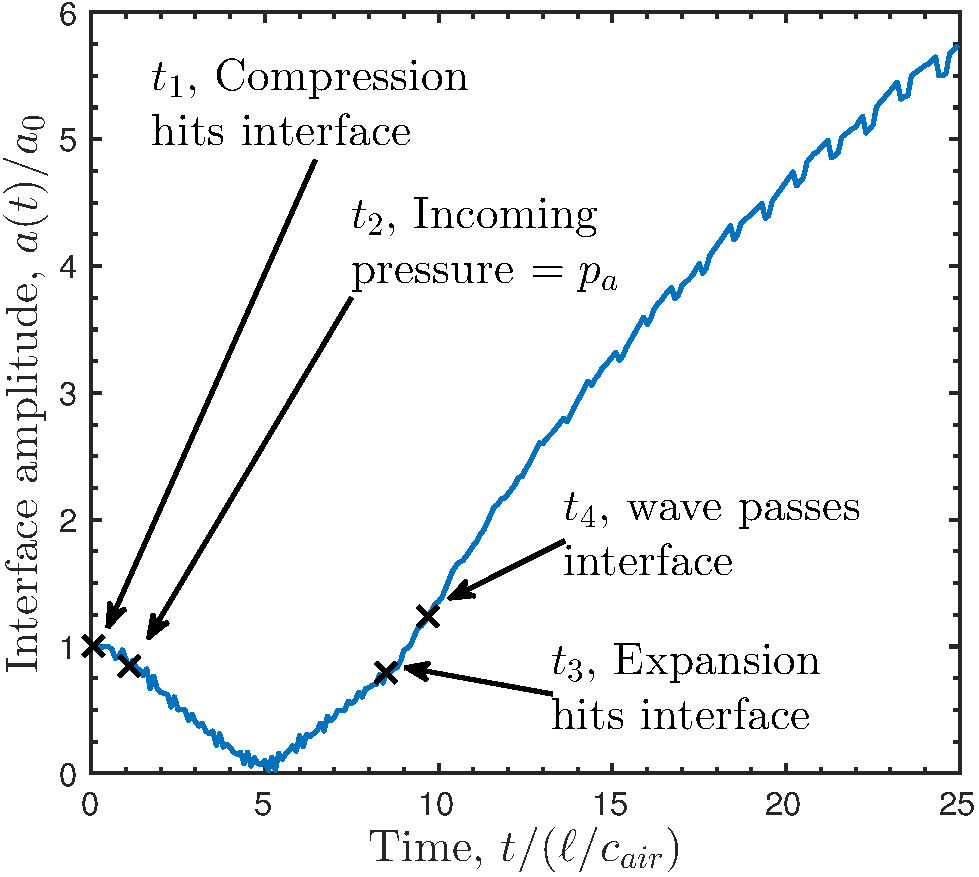
\includegraphics[width=\textwidth]{./figs/lung_figs/trapz10_intf_schematic.pdf}
    \begin{tikzpicture}%
      \node[anchor=south west,inner sep=0] (image) at (0,0) {
        \includegraphics[width=\textwidth]{./figs/lung_figs/trapz10_intf_schematic_24-May-2017.pdf}
      };%
      \begin{scope}[x={(image.south east)},y={(image.north west)}]%
        %\node[font=\small,right] at (0.85,0.2) {(a)};%
        \node[font=\small,align=center] at (0.0,1.0) {(a)};%
      \end{scope}%  
    \end{tikzpicture}%
    \phantomcaption
    \label{fig:trapz10_interface25}
  \end{subfigure}
  ~
  \begin{subfigure}[b]{0.45\textwidth}
    \centering
    \begin{tikzpicture}%
      \node[anchor=south west,inner sep=0] (image) at (0,0) {
        \includegraphics[width=1.025\textwidth]{./figs/lung_figs/trapz10_intf_t1000_24-May-2017.pdf}%
      };%
      \begin{scope}[x={(image.south east)},y={(image.north west)}]%
%        \node[font=\small,right] at (0.85,0.2) {(b)};%
        \node[font=\small,align=center] at (0.0,1.0) {(b)};%
      \end{scope}%  
    \end{tikzpicture}%
    \phantomcaption
    \label{fig:trapz10_interface1000}
  \end{subfigure}
  \caption{\label{fig:trapz10_interface}Interface perturbation amplitude history
    $a(t)/a_0$ for the baseline $p_a = 10$ MPa, $L=45\ell$ trapezoidal
    wave, for $t/(\ell/c) \leq 120$ \protect\subref{fig:trapz10_interface25}
    and $t/(\ell/c) \leq 5000$ \protect\subref{fig:trapz10_interface1000}. In
    \protect\subref{fig:trapz10_interface25}, times at which different
    stages of the incoming trapezoidal pressure wave first encounter
    the interface are indicated as $t_1$ (the compression), $t_2$ (the
    constant elevated pressure $p_a$), $t_3$ (the rarefaction), and
    $t_4$ (the return to ambient pressure).}
\end{figure}\par



\begin{figure}%
  \includegraphics[width=0.5\textwidth]{./figs/lung_figs/trapz10_bubble-spike_location_15-Sep-2017}
  \caption{\label{fig:trapz10_bs_location}$y$-locations of the bubble and spike for the baseline
    $p_a = 10$ MPa, $L=45\ell$ trapezoidal wave, during and shortly after the
    wave-interface interaction. By definition, the bubble is the top
    (solid, blue) curve and the spike is bottom (red, dashed)
    curve. Black, dotted line: $t_\Gamma$, as defined by the minimum
    bubble location.}  
\end{figure}%




The most important contribution of linear acoustics is the interface
translation (downward on the contour plots) during the interaction
with the wave; the overall interfacial perturbation evolution cannot
be explained solely by this principle. The combined effects of the
compression and the deformations occurring between the time the wave
travels from the perturbation peak to trough would yield a
perturbation amplitude change of approximately $0.01 a_0$. Linear
acoustics would further imply that the perturbation should no longer
evolve after the wave passage. It follows that nonlinear mechanisms
must drive the perturbation growth.
% As such, non-linear mechanisms are necessary to explain this
% observation, and as we will demonstrate in the upcoming sections, the
% directions of movement of the bubble and spike at $t_\Gamma$ and
% thereafter are consistent with what would be expected if the movement
% was driven by opposing baroclinic vortex pairs deposited by the wave.%
%
% \begin{comment}
%   It is further useful to analyze the growth of the bubble and spike
%   amplitude, as illustrated in for the baseline $p_a = 10$ MPa case
%   in Figure \ref{fig:trapz_bubble-spike_t1000}. Here we define the
%   bubble amplitude $a_b(t)$ and spike amplitude $a_s(t)$ as the
%   maximum and minimum $y-$location of the interface relative to the
%   location of an unperturbed flat interface also driven by the
%   wave. \hl(FIX THIS) The calculated growth of each goes as $t^n$
%   where $n=0.42 ( \text{bubble} ), 0.66 ( \text{spike} )$, and
%   $0.61 ( \text{bubble + spike} )$.%
% \end{comment}
% %
%
% \begin{figure}
%   \centering
%   \begin{subfigure}[t]{0.45\textwidth}
%     \centering
%     \includegraphics[height=0.8\textwidth]{./figs/lung_figs/bubble-spike_t1000_24-May-2017}
%     \caption{\label{fig:trapz_bubble-spike_t1000_unscaled} Constant scaling: $a(t)/\ell$}
%   \end{subfigure}
%   ~
%   \begin{subfigure}[t]{0.45\textwidth}
%     \includegraphics[height=0.8\textwidth]{./figs/lung_figs/bubble-spike_scaled_t1000_24-May-2017}
%     \caption{\label{fig:trapz_bubble-spike_t1000_scaled} Vortex strength scaling: $a(t)/\left(\frac{\Gamma_0}{s_0}\frac{\ell}{c}\right)$}
%   \end{subfigure}
%   \caption{The growth of the bubble (blue), spike (red), and sum of
%     the two (green) are shown for the baseline $p_a = 10$ MPa
%     trapezoidal wave case for $t \leq
%     5000$. \subref{fig:trapz_bubble-spike_t1000_unscaled} shows the
%     amplitudes $a(t)$ scaled by a constant
%     $\ell$. \subref{fig:trapz_bubble-spike_t1000_scaled} shows the
%     interface amplitude after the phase inversion scaled by
%     $\Gamma_0/s_0$, the circulation per unit arc length at
%     $t_\Gamma$. To facilitate the comparison, the time origin has been
%     shifted such that the instant the phase inverts occurs
%     simultaneously in each case. The dashed lines above the curves at
%     late times corresponds to power law growth with time.}
%   \label{fig:trapz_bubble-spike_t1000}
% \end{figure}
%%%%%%%%%%%%%%%%%%%%%%%%%%%%%%%%%%%%%%%%%%%%%%%%%%%%%%%%%%%%%%%%%% 
%%%%%%%%%%%%%%%%%%%%%%%%%%%%%%%%%%%%%%%%%%%%%%%%%%%%%%%%%%%%%%%%%% 
%%%%%%%%%%%%%%%%%%%%%%%%%%%%%%%%%%%%%%%%%%%%%%%%%%%%%%%%%%%%%%%%%% 
%%%%%%%%%%%%%%%%%%%%%%%%%%%%%%%%%%%%%%%%%%%%%%%%%%%%%%%%%%%%%%%%%% 
\subsubsection{Vorticity-based description of the perturbation growth}
\label{subsubsec:vorticity_growth}

The results presented in the previous section demonstrate that the
perturbation amplitude grows well after the incident wave has
traversed the interface, driven by a mechanism that cannot be
explained by conventional linear acoustics.  During interaction with
the interface, the pressure differential (due to the geometrical
perturbation) over a short distance applies a torque on fluid
particles along the interface, thus generating rotation (baroclinic
vorticity). Such effects would be of higher-order and thus negligible
for acoustic waves encountering small density variations; in the
present problem, however, the pressure and density change by
significant amounts over short distances, thus giving rise to
substantial gradients dominating otherwise first-order (acoustic)
effects.  For these reasons, we examine the perturbation growth in
terms of vorticity, $\boldsymbol{\omega}=\nabla\times\boldsymbol{u}$,
whose evolution in two dimensions is given by
\begin{align} \label{eq:vorticity_euler}
  \frac{\partial \boldsymbol{\omega}}{\partial t}+\left(\boldsymbol{u}\cdot\nabla\right)\boldsymbol{\omega} =% 
  - \boldsymbol{\omega}\left(\nabla\cdot\boldsymbol{u}\right) + \frac{\nabla\rho\times\nabla p}{\rho^2}.%
\end{align}
The high impedance mismatch and relatively low dilatation at the wave
amplitudes of interest make the first term on the right-hand side
(dilatation) essentially negligible compared to the last term
(baroclinic), which is large given the nearly discontinuous density
gradient and the significant pressure variations over relatively short
lengths; Appendix \ref{sec:oom_analysis} quantitatively supports this
claim.  Figure \ref{fig:vorticity_snapshots} depicts vorticity
contours at $t/(\ell/c) = 4.75, 47.5, 475,$ and $1424$, for the baseline
case. At time zero, there is no vorticity in the domain. Frame 1 shows
that near the end of the compression-interface interaction a vortex
sheet exists along the interface, with negative vorticity between
$x/\ell\in[0.0,0.5]$ and positive vorticity between
$x/\ell\in[0.5,1.0]$. The vorticity appears to be primarily in the air
as the interface location (black line) is taken to be the $\alpha=0.5$
volume fraction isoline. By frame 2, the initially deposited vorticity
has driven the perturbation peak downward such that the phase is now
reversed during the passage of the rarefaction. As a consequence of
this phase reversal, most of the vorticity deposited by the
rarefaction has the same sign as the distribution generated by the
compression, despite the corrugation of the interface. If the interface had remained undeformed, the vorticity
deposited by the rarefaction would have been opposite sign and thus
act to reduce that due to the compression.  Instead, the enhanced
vorticity gives rise to a clockwise (left-half domain) and
counter-clockwise (right-half domain) vortex pair driving the spike to
form at $x/\ell=0.5$. Over time, the vorticity contours become fainter,
but appear to spread over a larger region.
\begin{figure}
  \centering
  % 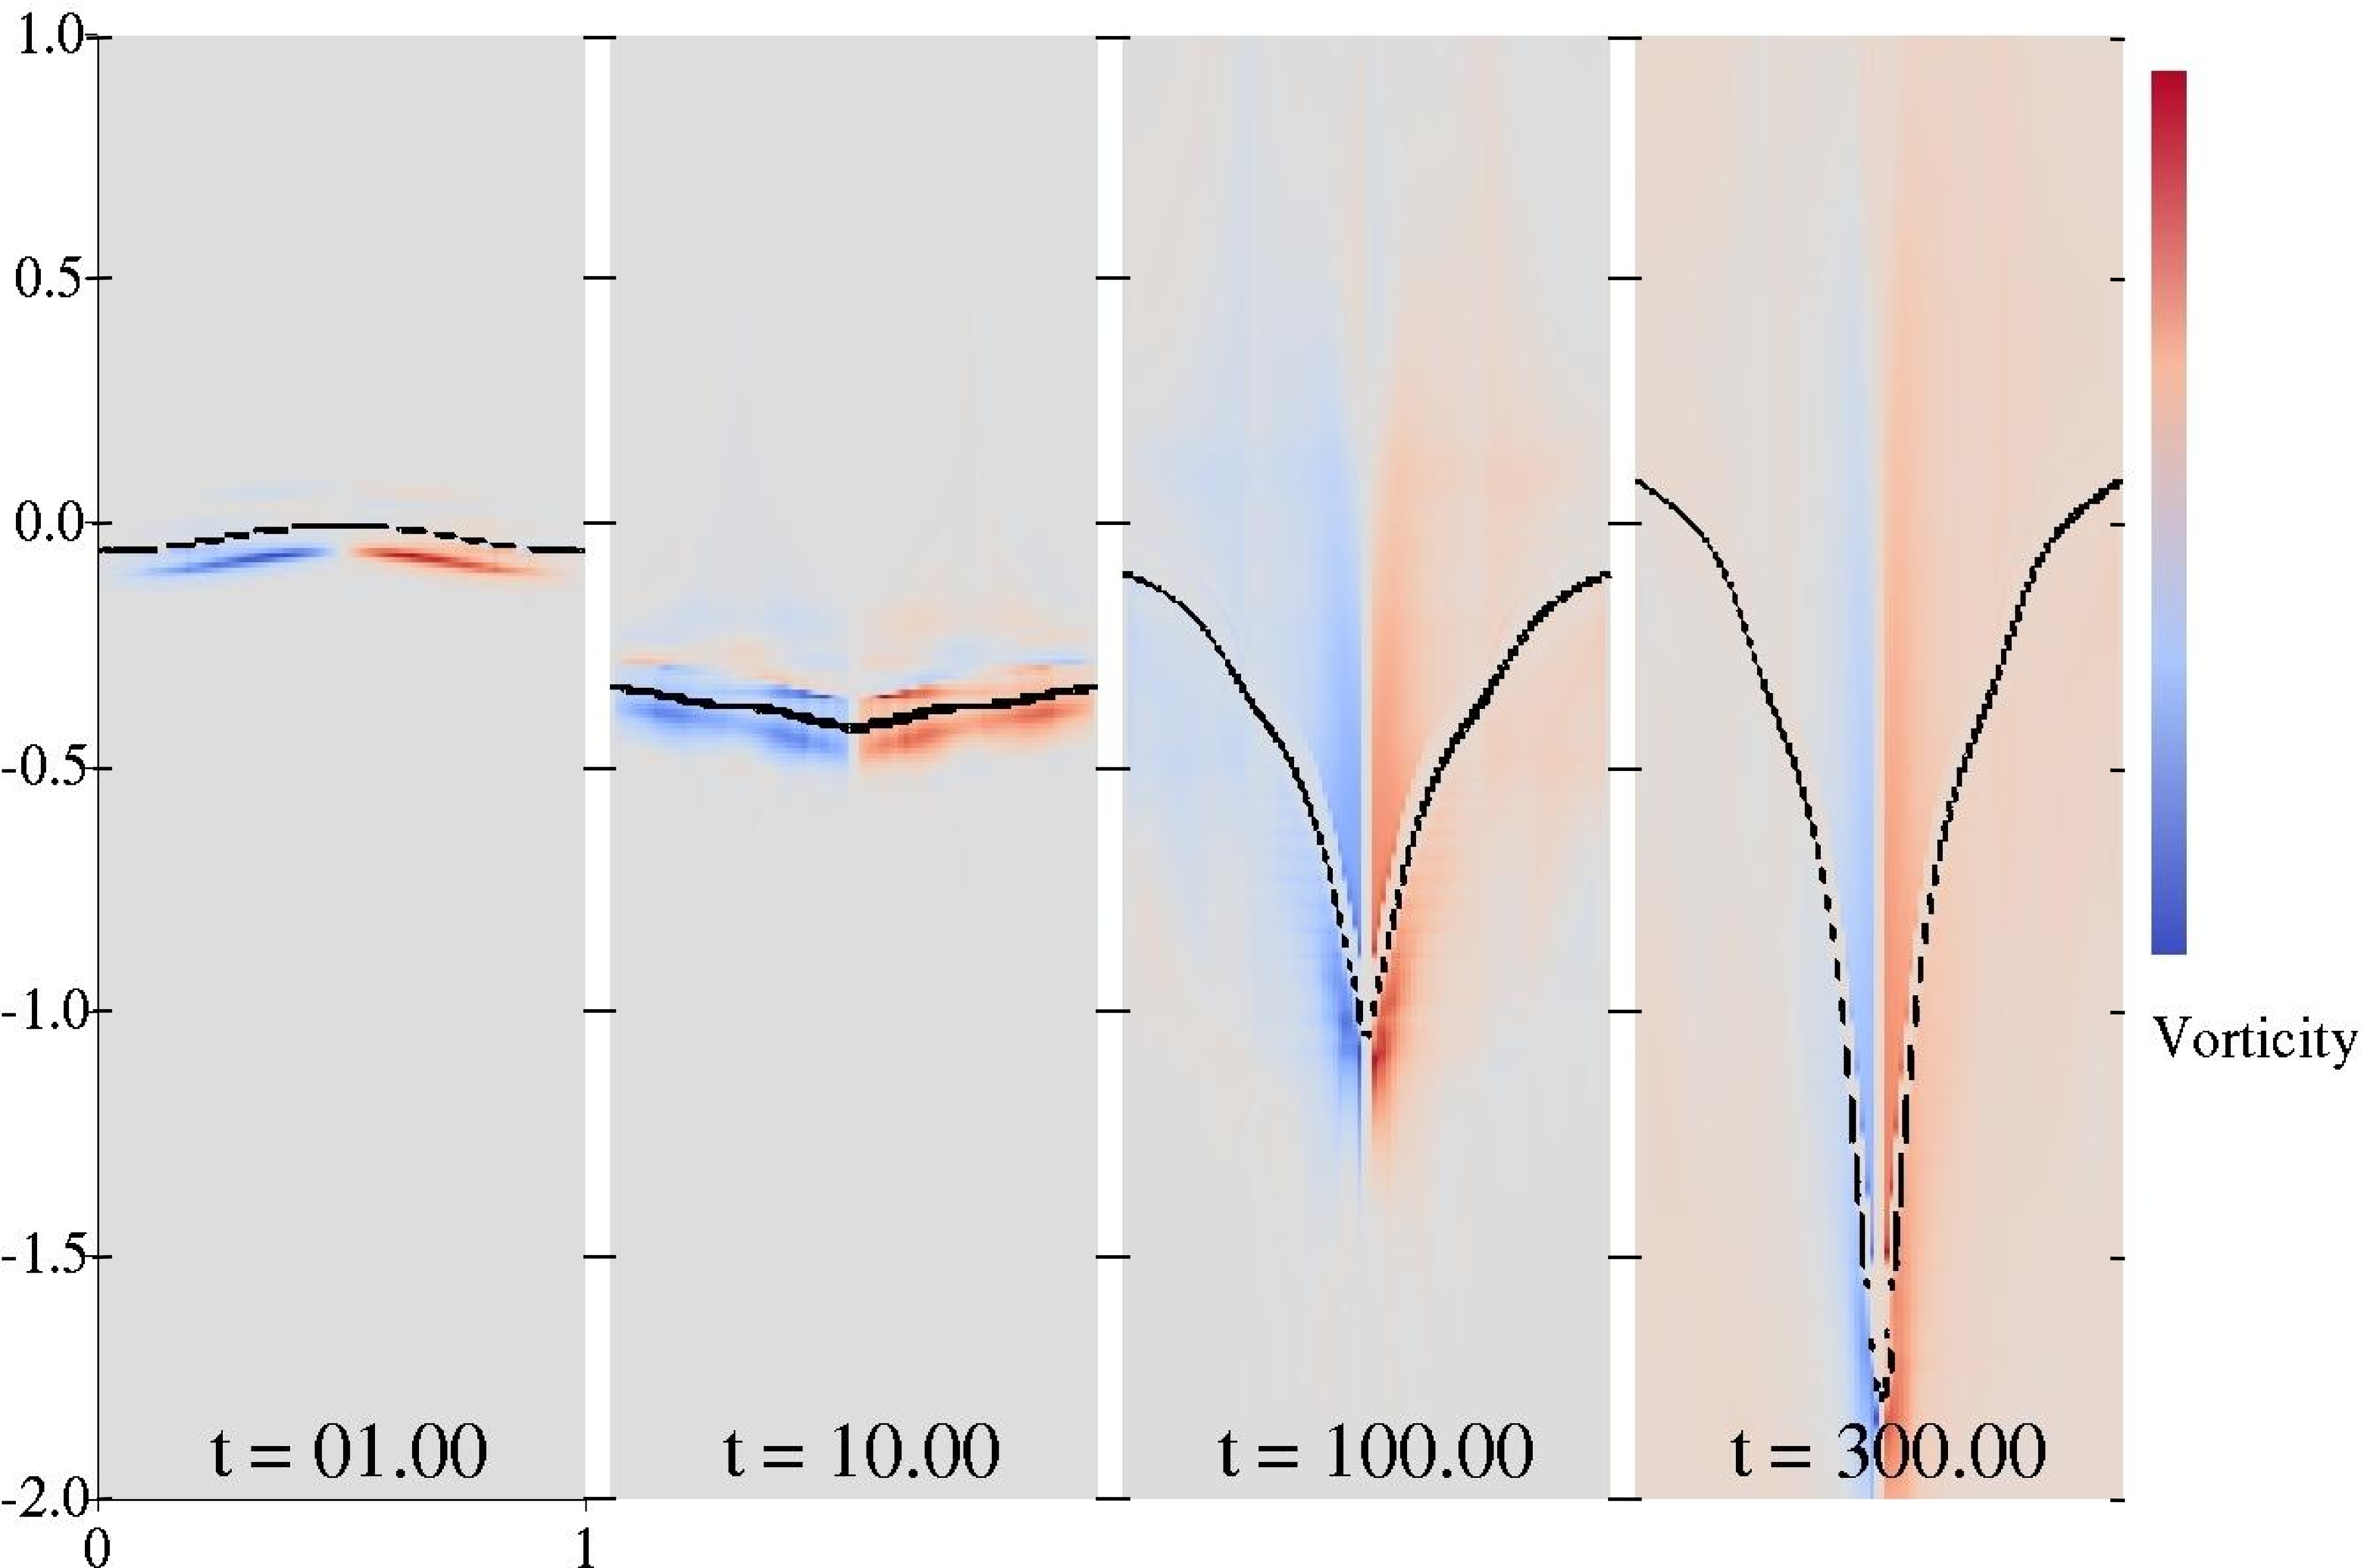
\includegraphics[width=0.9\textwidth]{./figs/lung_figs/snapshots_vorticity_t1}
  \includegraphics[width=0.98\textwidth]{./figs/lung_figs/vorticity_snapshot_fixcbar_mat_25-Sep-2017}
  \caption[The evolution of the vorticity] {Vorticity contours at $t/(\ell/c) =
    4.75, 47.5, 475$ and $1424$ for the baseline $p_a = 10$ MPa, $L=45
    \ell$ trapezoidal wave case. Black solid line: $\alpha=0.5$ volume
    fraction isoline; black dashed line: initial mean interface location.}
  \label{fig:vorticity_snapshots}
\end{figure}

During the interface evolution, the vorticity redistributes itself
along the interface. To quantify this behavior, we plot in Fig.
\ref{fig:vorticity_distribution} the cumulative vorticity (in $y$)
along the interface, $ \int_{-\infty}^{+\infty} \tilde{\omega}(x,y) dy
$, where $\tilde{\omega} = \omega$ for $0 < \alpha < 1$ and is
otherwise zero (in pure water or air). Initially, the vorticity is smooth and nearly
sinusoidal, as expected \citep{Samtaney1994}.  During the
phase reversal process, the vorticity peaks move toward
$x/\ell=0.5$. Given the geometry at the time when the rarefaction
arrives, a second peak in the vorticity distribution is observed near
$x/\ell=0.0$, $1.0$ at $t/(\ell/c)=47.5$. Though apparently fainter in the
contour plots, the vorticity is clearly concentrated near the spike,
driving the heavy fluid into the light one.

\begin{figure}
  \centering
  \includegraphics[width=0.5\textwidth]{./figs/lung_figs/vorticity_distribution_25-Sep-2017}
  \caption{Cumulative vorticity (in $y$) along the interface,
    $ \int_{-\infty}^{+\infty} \tilde{\omega}(x,y) dy $, where
    $\tilde{\omega} = \omega$ for $0 < \alpha < 1$ and is otherwise
    zero (in pure water or air), at $t/(\ell/c)=4.75$ (blue, solid), $47.5$
    (red, dashed), $475$ (green, dotted), and $1424$ (purple,
    dashed-dotted).}
  \label{fig:vorticity_distribution}
\end{figure}


For a more quantitative global measure of vorticity, we consider the
circulation produced in the right-half domain (the left is equal and
opposite by symmetry) for the baseline case in Fig.
\ref{fig:trapz10_circ_schematic}. The same times at which different
stages of the incoming trapezoidal pressure wave first encounter the
interface are indicated on this figure. From $t_1$ to $t_2$ (during
the interaction of the compression with the interface), positive
vorticity (circulation) is deposited given the direction of the
density and pressure gradients. This circulation increase is linear
since the pressure and density gradients are constant over the
interaction interval. Other than small changes due to transverse wave
reflections, the circulation remains essentially constant until $t_3$,
at which point the leading edge of the rarefaction encounters the
interface. Since the phase has reversed at $t_p$, the deposited
vorticity is of the same sign (i.e., positive) as that deposited by
the compression, such that the circulation approximately doubles by
the time the trailing end of the rarefaction arrives at
$t_4$. Thereafter, any changes in vorticity after this point, are no longer due to the
primary incoming wave. The decrease in circulation observed after the
wave passage is due to the intersection of the transverse reflections
of the rarefaction (now compressions) near the bubble, while the
late-time increase is attributed to the acceleration of the heavy
fluid into the light one as the spike penetrates the air, which is a
form of secondary baroclinic vorticity generation \citep{Peng2003}.

\begin{figure}
  \centering
  \begin{subfigure}[b]{0.48\textwidth}
    \centering
    \begin{tikzpicture}%
      \node[anchor=south west,inner sep=0] (image) at (0,0) {
        \includegraphics[width=\textwidth]{./figs/lung_figs/trapz10_circ_schematic_24-May-2017.pdf}
      };%
      \begin{scope}[x={(image.south east)},y={(image.north west)}]%
        \node[font=\small,align=center] at (0.0,1.0) {(a)};%
        % \node[font=\small,right] at (0.85,0.2) {(a)};%
      \end{scope}%  
    \end{tikzpicture}%
    \phantomcaption
    \label{fig:trapz10_circ_schematic_t25}
  \end{subfigure}
  ~
  \begin{subfigure}[b]{0.48\textwidth}
    \centering
    \begin{tikzpicture}%
      \node[anchor=south west,inner sep=0] (image) at (0,0) {
        \includegraphics[width=\textwidth]{./figs/lung_figs/Gamma_t1000_24-May-2017.pdf}
      };%
      \begin{scope}[x={(image.south east)},y={(image.north west)}]%
        \node[font=\small,align=center] at (0.0,1.0) {(b)};%
%        \node[font=\small,right] at (0.85,0.2) {(b)};%
      \end{scope}%  
    \end{tikzpicture}%
    \phantomcaption
    \label{fig:trapz10_circ_schematic_t1000}
  \end{subfigure}
  % 
  \caption{Circulation history for the right-half domain for the
    baseline $p_a = 10$ MPa, $L = 45 \ell$ trapezoidal wave case, for
    $t/(\ell/c) \leq 120$ \protect\subref{fig:trapz10_interface25} and $t/(\ell/c) \leq
    5000$ \protect\subref{fig:trapz10_interface1000}. In \protect\subref{fig:trapz10_interface25}, times at which
    different stages of the incoming trapezoidal pressure wave first
    encounter the interface are indicated as $t_1$: the compression;
    $t_2$: the constant elevated pressure $p_a$; $t_3$: the rarefaction;
    $t_4$: the return to ambient pressure.}
  \label{fig:trapz10_circ_schematic}
\end{figure}%





















%
%At $t_\Gamma=9.4$ nearly the entire interface region
%$(\alpha \leq 0.98)$ is subject to positive pressure.
% At $t_\Gamma=9.4$ $(\alpha \geq 0.65)$ is subjected to negative pressure gradient in y-direction.
% $(\alpha < 0.65)$ is subjected to no pressure gradient in y-direction.
%
%\subsubsection{Circulation-driven, late-time growth of the interface}


\subsection{Dependence of the perturbation growth on the wave amplitude}
\label{subsec:amp_dependence}%
\subsubsection{General Observations}
\label{subsubsec:general_observations}
Since the perturbation growth is driven by residual baroclinic
vorticity deposited by the interaction of the ultrasound wave with the
interface, it follows that the growth rate increases if more vorticity
is deposited. Thus, holding all other parameters fixed, we anticipate
the perturbation amplitude growth rate to increase with increasing
wave amplitude given that the baroclinic term is proportional to the
pressure difference. This behavior is confirmed by Fig.
\ref{fig:trapz_interface_acirc}, which shows the amplitude and
circulation histories for wave amplitudes ranging from $5.0$ to $12.5$
MPa; to help analyze the results, Table \ref{tab:circ} lists the
circulation at times $t_{1-4}$.  As expected, after the initial
transient, the late-time growth rate increases with increasing
pressure amplitude.  The circulation at the different $t_i$ follow a
consistent behavior, as the values increase with increasing pressure
amplitude. At $t_2$, we observe that the circulation deposited by the
compression increases at a nearly constant rate with pressure
amplitude, consistent with the fact that the time rate of change of
the circulation is proportional to the baroclinic term, itself
proportional to the pressure difference. From $t_2$ to $t_3$ and $t_3$
to $t_4$, the rise in circulation generally increases with increasing
amplitude, except for the 5 MPa wave between $t_3$ to $t_4$. In this
latter case, there is a decrease in circulation, due to the fact that
phase inversion has not occurred by the time the rarefaction
encounters the interface.  After $t_4$, we observe that both the
decrease and late-time rise in circulation depend on the pressure
amplitude; greater amplitudes lead to greater changes.  In the $12.5$
MPa case, the circulation appears to decrease at very late times
($t\geq4000$). This behavior is caused by round-off level errors
accumulating over the course of this long simulation, thus breaking
the left-right symmetry of the simulation \citep{Movahed2013}.

\begin{figure}
  \centering
  \begin{subfigure}[t]{0.48\textwidth}
    \centering
    \begin{tikzpicture}%
      \node[anchor=south west,inner sep=0] (image) at (0,0) {
        \includegraphics[width=\textwidth]{./figs/lung_figs/a0_t1000_25-Sep-2017}
      };%
      \begin{scope}[x={(image.south east)},y={(image.north west)}]%
        \node[font=\small,align=center] at (0.0,1.0) {(a)};%
%        \node[font=\small,right] at (0.85,0.9) {(a)};%
      \end{scope}%  
    \end{tikzpicture}%
    \phantomcaption
    \label{fig:trapz_interface_t1000}
  \end{subfigure}
  ~
  \begin{subfigure}[t]{0.48\textwidth}
    \centering
    \begin{tikzpicture}%
      \node[anchor=south west,inner sep=0] (image) at (0,0) {
        \includegraphics[width=1.05\textwidth]{./figs/lung_figs/Circulation_t1000_25-Sep-2017}
      };%
      \begin{scope}[x={(image.south east)},y={(image.north west)}]%
        \node[font=\small,align=center] at (0.0,0.945) {(b)};%
        %\node[font=\small,right] at (0.85,0.88) {(b)};%
      \end{scope}%  
    \end{tikzpicture}%
    \phantomcaption
    \label{fig:trapz_circ_t1000} 
  \end{subfigure}
  % 
  \caption[The interface amplitude and circulation for long time and
    multiple wave amplitudes]{Histories of the interface amplitude
    \subref{fig:trapz_interface_t1000} and circulation
    \subref{fig:trapz_circ_t1000} for trapezoidal wave cases with
    $L=45\ell$, $p_a = 5.0$ (blue, solid), $7.5$ (red, dashed), $10.0$ (green, dotted), and
    $12.5$ (purple, dashed-dotted) MPa, for $t/(\ell/c)\leq 5000$.}
  \label{fig:trapz_interface_acirc}
\end{figure}



\begin{table}
\centering
\caption{Circulation during the wave-interface interaction.}
\label{tab:circ}
\begin{tabular}[t]{L{0.15\linewidth} L{0.1\linewidth} L{0.1\linewidth} L{0.1\linewidth} L{0.1\linewidth} }
\toprule
&\multicolumn{4}{c}{$\Gamma(t_i)/(\ell c) \times 10^{3}$}\\
$p_a$ (MPa) &$t_1$&$t_2$&$t_3$&$t_4$\\% t = 0, 5.22,40.36,47.00
\midrule
5.0&0&3.3&3.8&2.9\\
7.5&0&5.0&6.0&8.7\\
10.0&0&6.8&8.8&18.0\\
12.5&0&8.5&11.9&30.5\\
\bottomrule
\end{tabular}
\end{table}%
\begin{comment} %time [circ (t1-4)]
5.00 MPa         0    0.0000    0.3349    0.3834    0.2949
7.50 MPa    5.2227    0.0000    0.5041    0.6006    0.8704
10.0 MPa   40.3573    0.0000    0.6758    0.8814    1.7981
12.5 MPa   47.0044    0.0000    0.8529    1.1856    3.0511
\end{comment}






\subsubsection{Late time scaling of the perturbation amplitude}
The smooth and monotonous behavior of the perturbation amplitude
growth suggests that a more general scaling describing its dependence
on the pressure amplitude may exist.  Clearly, the perturbation growth
is related to the circulation $\Gamma$. As the perturbation grows, the
vorticity redistributes itself along the interface, such that
dependence on the interface length $s$ and the initial wavelength
$\ell$ are expected. Finally, given that the waves traverse the
interface over a finite duration, dependence on the sound speed $c$ is
expected. Thus, the dependence of the amplitude on these variables can
be formulated as a dimensional analysis problem:
\begin{align}
  \label{eq:dimensional_amplitude}
  a(t)=f(\Gamma, s, \ell, c; t) \quad \Rightarrow \quad
  \frac{a(t)}{\ell} = G\left(\frac{\Gamma}{\ell c}, \frac{s}{\ell};
  \frac{t}{\ell/c}\right),
\end{align}
where $\ell$ and $c$ are used for non-dimensionalization. We note that
there is likely an Atwood number dependence, but since the density
fields do not significantly change we ignore this parameter here. Well
after the wave passage (e.g., for $t\gtrsim 500$), the circulation no
longer changes significantly (except perhaps in the $p_a = 12.5$ MPa
case, where the circulation changes up to approximately 30\%), as
there is no dominant mechanism to affect it. However, as the interface
deforms and elongates (i.e., $s(t)$ increases), the vorticity gets
redistributed along the interface.  The circulation density
$\Gamma / s$ is thus a relevant quantity describing the vortex
dynamics \cite[]{Pozrikidis2000}. As observed in Section
\ref{subsubsec:vorticity_growth}, the baroclinic vorticity is the
dominant contributor to the interface perturbation growth after
$t_\Gamma$. Thus, we expect the perturbation amplitude to depend on
the circulation density at this time, which we define
$\Gamma(t_\Gamma)/s(t_\Gamma) = \Gamma_0 / s_0$. It therefore follows
that
% 
\begin{align}
  \label{eq:dimensionless_groups}
  \frac{a(t)}{\ell}=F\left(\frac{\Gamma_0}{s_0 c}, \frac{t c}{\ell} \right).
\end{align}
% 
% As suggested by the observed behavior in Figure
% \ref{fig:trapz_interface_acirc} and Table \ref{tab:circ}, 
Finally, we hypothesize that the perturbation growth scales linearly
with the circulation density, such that
% 
\begin{align}
  \label{eq:dimensionless_relationship}
  \frac{a(t)}{\ell}=\frac{\Gamma_0}{s_0 c}\mathcal{F}\left(\frac{t c}{\ell} \right).
\end{align}
% 
To verify this hypothesis, we plot the perturbation amplitude $a(t)$
scaled by the circulation density at $t_\Gamma$ in Fig.
\ref{fig:trapz_interface_t1000_scaled}. To facilitate the comparison,
the time origin has been shifted by $t_p$ such that the instant the
phase inversion has been synchronized for all cases.  Two
observations stand out. First, the scaled growths collapse onto what appears to be
a single curve at sufficiently late times. Second, this curve appears to asymptote to a
constant slope, thus exhibiting a power-law behavior
$\mathcal{F} = (tc/\ell)^n$. To compute $n$, we write
\begin{align}
  \label{eq:log_a}
  \ln\left[(a(t-t_p) / \left(\frac{\Gamma_0}{s_0}\frac{\ell}{c}\right)\right] = b + n\ln\left[(t-t_p)/(\ell/c)\right],
\end{align}
where $t_p$ is phase-reversal time and $b$ is the $y-$intercept of the
best fit line, which depends on the value of
$a(t-t_p) / \left(\frac{\Gamma_0}{s_0}\frac{\ell}{c}\right)$ when the
interface growth becomes asymptotic. By applying linear regression to
the data for $(t-tp) \geq 2000$, we determine the best fit values for
$n$ in a least squares sense. We find that $n \approx 3/5$, as
illustrated in Table \ref{tab:growth_exponents}. Though difficult to
distinguish in Fig. \ref{fig:trapz_interface_t1000_scaled}, the
$p_a=12.5$ MPa case exhibits a slightly higher time exponent, with $n$
closer to $2/3$; this discrepancy may be due to the fact that
circulation, even at late times, still changes in a non-negligible
fashion in this case. We note however that this amplitude falls beyond
those typically used in clinical diagnostic ultrasound. We also remark
that grid independence is not achieved on the current grid, such that
the actual value of the exponent may change slightly as finer grids
are used; on the other hand, the collapse of the data does not appear
to depend on the grid spacing.
%
\begin{table}
\centering
\caption{Interface amplitude growth time exponents, where $\frac{a(t)}{\ell}\sim t^n$.}
\label{tab:growth_exponents}
\begin{tabular}[t]{L{0.15\linewidth} L{0.13\linewidth} }
\toprule
$p_a$ (MPa) & $n(t\geq2000)$\\
\midrule
5.0&0.61\\
7.5&0.59\\
10.0&0.61\\
12.5&0.66\\
\bottomrule
\end{tabular}
\end{table}%
%
\begin{figure}
  \centering
 \includegraphics[width=\textwidth]{./figs/lung_figs/intf_amp_t1000_25-Sep-2017}
  \caption{Interface amplitude scaled by circulation density at
    $t_\Gamma$ for the trapezoidal wave cases with $L=45\ell$, $p_a =
    5$ (blue, solid), $7.5$ (red, dashed), $10$ (green, dotted), and $12.5$ (purple, dashed-dotted)
    MPa. Time is synchronized based on phase inversion. Black dashed
    line: power-law growth as $t^{3/5}$.}
  \label{fig:trapz_interface_t1000_scaled}
\end{figure}
%

\subsubsection{Late time scaling of the interfacial length}
The tenfold to hundredfold perturbation amplitude growth is
accompanied by a corresponding increase in interfacial length
$s$. This quantity is important for the dynamics of the vortex sheet
produced along the interface by the ultrasound passage
\citep{Pozrikidis2000}; vortex sheet dynamics have in fact been
explored in the context of the Rayleigh-Taylor instability
\citep{Tryggvason1988}. In such analysis, the quantity of interest is
the circulation density $\Gamma / s$.  We expect this quantity to depend on the wave amplitude
$p_a$, the initial wavelength $\ell$, the density and sound speed of
the liquid, $\rho$ and $c$, respectively. Following a dimensional
analysis process similar to that in the previous section, we find that
the inverse of the circulation density (in other words: the
interfacial length scaled by instantaneous circulation) bears the
following dependence on the relevant dimensionless parameters:%
%
\begin{align}
  \frac{s(t)}{\Gamma(t)}c = \psi\left(\frac{p_a}{\rho c^2},\frac{tc}{\ell}\right).%
\end{align}
%
Given that the growth is baroclinic, we hypothesize that the
circulation scales linearly with pressure amplitude, such that%
%
\begin{align}
  \frac{s(t)}{\Gamma(t)/c} = \frac{\rho c^2}{p_a}f\left(\frac{tc}{\ell}\right).%
\end{align}%
To determine the time dependence of the interfacial length, we plot in
Fig. \ref{fig:trapz_scp_t1000} the time histories of the interfacial
length and scaled interfacial length. Again, time is synchronized
based on phase inversion. As for the amplitude, the growth rate of the
length increases with pressure amplitude. Furthermore, with the
exception of the $p_a = 5$ MPa case, our simple scaling collapses the
interfacial length onto a single curve after a sufficiently long time
($t\gtrsim 500$). The collapsed curve exhibits a power-law dependence
on time $f=(tc/\ell)^m$, where $m \approx 1/2$ for $p_a = 7.5, 10$ and
$12.5$ MPa. This scaling confirms that the interfacial deformations
are governed by the dynamics of the vortex sheet produced by the
ultrasound interaction. The result from the $p_a = 5$ MPa case does
not follow the same behavior for two main reasons. First, the
rarefaction encounters the interface during phase inversion, at which
point the interface is essentially flat.  Thus, the vorticity
contribution is negligible; nevertheless, the rarefaction accelerates
the interface and increases its length, thus decreasing the
circulation density. As a result, the geometry at $t_p$ is different
from that observed in the other cases.  Second, $s/\Gamma$ has yet to
achieve its asymptotic behavior.  However, running the simulation to
asymptotic behavior would be prohibitively expensive from a
computational standpoint.

We highlight the different dependence of the perturbation amplitude
and interfacial length on circulation. The growth of the former is
dictated by the geometry and the amount of circulation at the end of
the interaction. Thus, the instantaneous circulation at that time is
sufficient to describe the growth. On the other hand, the interfacial
length depends on the details of the vortex sheet dynamics. Thus, the
interfacial length is sensitive to the instantaneous circulation and
in fact local vorticity.
%
\begin{figure}
  \centering
  \begin{subfigure}{0.45\textwidth}
    \begin{tikzpicture}%
      \node[anchor=south west,inner sep=0] (image) at (0,0) {
        \includegraphics[height=\textwidth]{./figs/lung_figs/s_t1000_25-Sep-2017}
       };%
       \begin{scope}[x={(image.south east)},y={(image.north west)}]%
         \node[font=\small,align=center] at (0.0,1.0) {(a)};%
%         \node[font=\small,right] at (0.82,0.17) {{(a)}};%
       \end{scope}%  
     \end{tikzpicture}%
     \phantomcaption
     \label{fig:trapz_scp_t1000_unscaled}
   \end{subfigure}
   ~~~
   \begin{subfigure}{0.45\textwidth}
     \begin{tikzpicture}%
       \node[anchor=south west,inner sep=0] (image) at (0,0) {
         \includegraphics[height=\textwidth]{./figs/lung_figs/scp_t1000_25-Sep-2017}
       };%
       \begin{scope}[x={(image.south east)},y={(image.north west)}]%
         \node[font=\small,align=center] at (0.0,1.0) {(b)};% 
%        \node[font=\small,right] at (0.15,0.92) {{(b)}};%
       \end{scope}%  
     \end{tikzpicture}%
     \phantomcaption
     \label{fig:trapz_scp_t1000_scaled} 
  \end{subfigure}
  \caption{Histories of the
    interfacial length \subref{fig:trapz_scp_t1000_unscaled} and
    scaled interfacial length \subref{fig:trapz_scp_t1000_scaled} for
    the trapezoidal wave cases with $L=45\ell$, $p_a = 5$ (blue, solid), $7.5$
    (red, dashed), $10$ (green, dotted), and $12.5$ (purple, dashed-dotted) MPa. Time is synchronized
    based on phase inversion. Black dashed line: power law growth as
    $t^{1/2}$.}
  \label{fig:trapz_scp_t1000}
\end{figure}
% 





\subsection{\label{subsubsec:transient}Dependence of the growth on the wave duration}%
The results from the previous sections indicate that the interface
morphology during the interaction of the rarefaction with the
interface plays a key role in the dynamics.  If the interface has
undergone phase inversion by the time the rarefaction has arrived,
vorticity of the same sign as that due to the compression is
deposited, thus enhancing the growth.  On the other hand, if the
rarefaction arrives before the phase has inverted, vorticity of the
opposite sign is deposited and counteracts the vorticity initially
deposited by the compression. In the limit where the rarefaction
immediately follows the compression, zero net vorticity would be
deposited \emph{only if the interface has not deformed}, thus leading
to no growth.  The amount of baroclinic vorticity deposited by the
rarefaction depends on the interface morphology at the time of
interaction, described by the sine of the angle between density and
pressure gradients, such that the effect of the rarefaction on the
interface perturbation growth depends heavily on the time-dependent
features of the wave. To examine this behavior, we hold the pressure
amplitude constant at $p_a = 10$ MPa and vary the time (or length $L$)
between the compression and rarefaction. The corresponding amplitude
and circulation histories are shown in Fig.
\ref{fig:trapz_circ_interface_multi-lag}.  For the two longest waves,
$L=35\ell$ and $45\ell$, the rarefaction encounters the interface well
after phase inversion. In these cases, the rarefaction deposits
additional vorticity of the same sign as that due to the compression
(e.g., positive vorticity in the right side of the domain) and
enhances growth. For the $L=30\ell$ case, the rarefaction impinges
upon the interface shortly after the interface phase-reversal, when
the interface is nearly flat. As a result, the pressure and density
gradients are nearly aligned and little additional circulation is
generated. Thus the growth is driven purely by the circulation
deposited by the compression. For shorter waves ($L \leq 25\ell$), the
rarefaction encounters the interface before the perturbation reverses
phase, thus reducing the circulation.  Among cases for which the
interface inverts phase before encountering the rarefaction, the
larger the instantaneous perturbation amplitude at the time of the
rarefaction, the greater the circulation generated, since the average
angle between the density and pressure gradients is greater. The same
is true when comparing cases for which the interface inverts its phase
before encountering the rarefaction.

These results suggest that by appropriately modulating the incoming
wave the perturbation growth could be controlled. This observation is
particularly important for waves for which the pressure returns to
its ambient value after the wave passage, which is the case for
acoustic waves in general by contrast to the conventional
shock-accelerated (Richtmyer-Meshkov instability) problem.

\begin{figure}
  \centering
  \begin{subfigure}{0.48\textwidth}
    \centering
    \begin{tikzpicture}%
      \node[anchor=south west,inner sep=0] (image) at (0,0) {
        \includegraphics[width=\textwidth]{./figs/lung_figs/interface_multi-lag_25-Sep-2017}
      };%
      \begin{scope}[x={(image.south east)},y={(image.north west)}]%
        \node[font=\small,align=center] at (0.0,1.0) {(a)};%
        %\node[font=\small,right] at (0.1,0.9) {{(a)}};%
      \end{scope}%  
    \end{tikzpicture}%
    \phantomcaption
    \label{fig:trapz_interface_multi-lag} 
  \end{subfigure}
  ~
  \begin{subfigure}{0.48\textwidth}
    \centering
    \begin{tikzpicture}%
      \node[anchor=south west,inner sep=0] (image) at (0,0) {
        \includegraphics[width=\textwidth]{./figs/lung_figs/circulation_multi-lag_legend_25-Sep-2017}
      };%
      \begin{scope}[x={(image.south east)},y={(image.north west)}]%
        \node[font=\small,align=center] at (0.0,1.0) {(b)};%
        %\node[font=\small,right] at (0.125,0.88) {{(b)}};%
      \end{scope}%  
    \end{tikzpicture}%
    \phantomcaption
    \label{fig:trapz_circ_multi-lag}%
  \end{subfigure}
  \caption[The interface and circulation dependence on wave
  duration]{Interface amplitude \subref{fig:trapz_interface_multi-lag}
    and circulation \subref{fig:trapz_circ_multi-lag} histories for
    the $p_a=10$ MPa trapezoidal wave case with $L=45\ell$ (blue, solid),
    $35\ell$ (red, dashed), $30\ell$ (green, dotted), $20\ell$ (purple, dashed-dotted),
    $15\ell$ (orange, with circles), $10\ell$ (yellow, with triangles).}
  \label{fig:trapz_circ_interface_multi-lag}
\end{figure}
%
%
%
%
% ============================== Conclusions =========================
%
\section{\label{sec:conclusions}Conclusions}
We investigated the interaction of an acoustic wave propagating in a
liquid and impinging upon a perturbed liquid-gas interface, as a model
for ultrasound interaction with alveoli, in consideration of lung
hemorrhage.  Despite selecting a simplified, yet relevant waveform
(trapezoidal, symmetric in time, returns to ambient conditions after
pressure rise) to facilitate the analysis, the results are
generalizable to more complex, continuous ultrasound waveforms.  For
waveform parameters relevant to the application, we observed that
acoustic waves in water lead to interface perturbation phase
inversion, followed by perturbation growth to amplitudes many times
larger than the initial value well after the wave passage. We further
characterized the dependence of the perturbation growth on the wave
amplitude and length.

We demonstrated that the mechanism driving the perturbation growth is
the torque generated by the misalignment of the pressure and density
differentials during the wave interaction, manifested by the
production of baroclinic vorticity along the interface.  This effect,
usually higher-order in acoustics, is dominant in our problem due to
the substantial pressure difference over a short length (megapascals
over millimeters), and the nearly discontinuous density
profile. Although the symmetric nature of the wave may suggest that
vorticity deposited by the compression should be exactly canceled by
that produced by the rarefaction, such an argument overlooks the
transient nature of the process, namely the fact that the baroclinic
torque drives the interface to deform during the passage of the
compression, during the time when the pressure amplitude is kept high, and
during the passage of the rarefaction. As a result, the alignment
between the pressure and density gradients is different during the
passage of the rarefaction, compared to that produced by the
compression. This result can be generalized to state that, except for
very special cases, waves interacting with an interface over a finite
duration and producing interface deformation generate net baroclinic
vorticity, whether the wave is symmetric in time or not.

An immediate consequence of the problem of interest is the observation
of two perturbation growth regimes, depending on whether phase
inversion has occurred by the time when the rarefaction reaches the
interface. If the phase has inverted, vorticity of the same sign as
that deposited by the compression is produced, thus leading to
enhanced growth; conversely, if phase has not yet inverted, vorticity
of the sign opposite that deposited by the compression is produced,
thus leading to reduced growth. Varying the amplitude and length of the
wave can push the dynamics from one regime to the other.  We also note
that at sufficiently high amplitudes the late time perturbation growth
obeys a power-law scaling. By considering the evolution of the
interfacial length and the vorticity redistribution along the
interface, we found that this result is consistent with a
vortex-sheet-based description of the interface dynamics. Finally, the
dependence of the results on the wave length suggests that
perturbation growth may be controlled by modulating the waveform.

This work is a step toward a fundamental understanding of the effects
of acoustically generated vorticity along liquid-gas interfaces. The
results suggest that significant strains may be imposed upon the
interface. To directly relate these findings to ultrasound-induced lung
hemorrhage, however, a more comprehensive description of the
tissue-lung rheology (viscoelastic properties) and geometry is
required, along with the use of application-specific waveforms.




\subsection*{Acknowledgements}

This work was supported in part by the National Science Foundation
Graduate Research Fellowship under NSF Grant Number DGE 1256260, and
under NSF grant 1253157 and NIH grant 4-R01-HL-116434-04. This work
used the Extreme Science and Engineering Discovery Environment
(XSEDE), which is supported by National Science Foundation grant
number ACI-1548562. The authors thank Prof. Douglas L. Miller for many
useful discussions.\nocite{Towns2014}


\appendix
\section{Order of magnitude analysis of vorticity dynamics}
\label{sec:oom_analysis}
To quantifiably compare the various mechanisms by which vorticity
changes in the flow, we perform an order of magnitude analysis on each
term of the vorticity transport equation
\eqref{eq:vorticity_euler}. Initially, there is no vorticity. Given
the present problem set-up, the only mechanism that can produce
vorticity is the baroclinic torque, which is clearly non-zero during
the interaction of the ultrasound wave with the interface since the
pressure (wave) and the density (interface) gradients are
misaligned. For this reason, we focus on the relative magnitude of
each term during the interaction time,
$\Delta t_a \approx 5\ell/c_{water}$, as the compression encounters
the interface. Since the average perturbation amplitude during the
interaction is sufficiently small ($\sim 0.96a_0$), we assume the
interface remains static and undeformed throughout the interaction,
such that the density gradient is approximately constant. We treat the
divergence and magnitude of curls/gradients of quantity $f$ as
$\sim \Delta f/ \Delta L$, where $\Delta L$ is the problem's
characteristic length scale. Since flow is driven by the acoustic wave
$\Delta p=\Delta p_a$, $\Delta u=\Delta u_a$, and
$\Delta \rho=\Delta \rho_a$, where the subscript $_a$ denotes acoustic
quantities. The quantities are related according to,
\begin{align}%
  \label{eq:acoustic_relations}%
  \Delta p_a=\pm\Delta u_a \rho c=c^2\Delta \rho_a.%
\end{align}
Since $a_0/\ell\ll 1$ (indicating small misalignment between
$\nabla \rho$ and $\nabla p$), we can approximate
$\sin \theta \approx \theta$. It thus follows that the magnitude of the
baroclinic term is
\begin{align}
  \label{eq:baroclinic_vorticity}%
  \norm{\frac{\nabla\rho\times\nabla p}{\rho^2}} =%
  |\nabla \rho||\nabla p||\sin\theta|=
  \orderof{\frac{\abs{\Delta \rho_I}}{\abs{\Delta L_I}}\frac{\abs{\Delta p_a}}{\abs{\Delta L_a}}\frac{1}{\abs{\rho}^2}\abs{\theta}}.%
\end{align}
where $\Delta \rho_I$ is the density jump across the interface,
$\Delta p_a$ is the pressure amplitude of the wave, $\Delta L_I$ is
the characteristic length of the interface (thickness) and
$\Delta L_a$ that of the wave (wavelength). Approximating the
vorticity as of equal magnitude to the baroclinic term, the dilational
term can be estimated as
\begin{align}
  \label{eq:compressible_advective_vorticity}%
  \norm{-\boldsymbol{\omega}\left(\nabla\cdot\boldsymbol{u}\right)} = %
  \orderof{%
  \frac{\abs{\Delta u_a}}{\abs{\Delta L_a}} \frac{\abs{\Delta \rho_I}}{\abs{\Delta L_I}}%
  \frac{\abs{\Delta p_a}}{\abs{\Delta L_a}} \frac{1}{\abs{\rho}^2}\abs{\theta}%
  }.%
\end{align}
%
Making use of Equation \eqref{eq:acoustic_relations}, the relative magnitude of the baroclinic to dilational terms is:
\begin{align} \label{eq:vorticity_comparison}
  \frac{\norm{\frac{\nabla\rho\times\nabla
  p}{\rho^2}}}{\norm{-\boldsymbol{\omega}\left(\nabla\cdot\boldsymbol{u}\right)}}
  \sim \orderof{\frac{\abs{c}}{\abs{\Delta u_a}}} = \orderof{\frac{\abs{\rho}}{\abs{\Delta \rho_a}}}%
\end{align}

To evaluate the above expressions for comparison with our
computational results, we consider our base trapezoidal wave case
where $p_a = \Delta p_a = 10$ MPa. The length scale associated with
the acoustic wave is the initial length of the pressure compression
$\Delta l_a=5\ell$. The initial interface length scale $\Delta L_i$,
defined as the thickness of the mixed layer from $\alpha=0.05$ to
$0.95$ volume fraction of water is estimated as
$\Delta L_i \approx 0.05\ell$. We approximate the order of $\theta$
based on its average value along a half-wavelength of the interface
for $a_0=0.03\ell$ such that the average value of
$\abs{\theta}\approx0.12$. evaluating expression
\eqref{eq:vorticity_comparison} we to find that
$\abs{c}/\abs{\Delta u_a}$=$\orderof{10^2}$ and thus expect that the relative
contribution of baroclinic to compressible/advective vorticity
generation is approximately of order $\orderof{10^2}$ at
$t = \Delta t_a \approx 5$.

To compare our computational results to the analysis we consider the
integral of the vorticity and vorticity generation terms over the
right-half domain,
\begin{align}
  \Gamma = \int_{A_{rh}} \omega \,dA_{rh},
\end{align}
where $\int_{A_{rh}} dA_{rh} =
\int_{-\infty}^{+\infty}\int_{\ell/2}^{\ell} \,dy\, dx$. Only the
right-half domain is considered because the total circulation over the
whole domain is zero due to symmetry. Circulation is chosen as the
quantity of comparison as it is a global quantity, which better
captures the overall vorticity dynamics than the vorticity at any
single point. As a single quantity rather than a field, it is also
simpler to compare the computational and analytical results. The
relative order of magnitude relationships obtained in
\eqref{eq:vorticity_comparison} are spatially independent and expected
to hold when integrated over the right-half domain. Accordingly we
evaluate the vorticity generation terms from our computational results
integrated over the right-half domain. At $t\approx5.0$ we find that %
\begin{comment}
  $$ \int_{A_{rh}} \left[\frac{\nabla\rho\times\nabla p}{\rho^2}\right]\,dA_{rh} / \int_{A_{rh}}\left[\left(\boldsymbol{u}\cdot\nabla\right)\boldsymbol{\omega}\right]\,dA_{rh}\approx 285=\orderof{10^2}$$
  and
\end{comment}
\begin{align}
  \frac{\int_{A_{rh}} \left[\frac{\nabla\rho\times\nabla p}{\rho^2}\right]\,dA_{rh}}%
  {\int_{A_{rh}} \left[-\boldsymbol{\omega}\left(\nabla\cdot\boldsymbol{u}\right)\right]%
  \,dA_{rh}}%\approx 145}
  =\orderof{10^2}.
\end{align}
% 
Hence the computational results and analysis are in agreement and
suggest that the vorticity is nearly entirely baroclinic.
% 

 
\bibliographystyle{jfm}
% note the spaces between the initials

\bibliography{./bibliography}

\end{document}

%%% local variables:
%%% mode: latex
%%% tex-master: 
%%% end:

